%
% This file is the code for an actual presentation I gave in 2013,          (mh)
% and is now used here to demonstrate the 'mh-presentation' document
% class. Comments are strategically placed to explain certain commands.
% Search for the string '(mh)' in this file to jump to those comments.
%
% To compile a document using this document class, LaTeX needs to be
% able to find the .cls files. So either register them with your LaTeX
% distribution, or put them in the same directory as your document.
% Moreover, you need to enable shell escape in the LaTeX engine, e.g.:
%
%     pdflatex -shell-escape presentation.tex
%
% Have fun!
%
% --- Michiel Helvensteijn (www.mhelvens.net)
%
%%%%%%%%%%%%%%%%%%%%%%%%%%%%%%%%%%%%%%%%%%%%%%%%%%%%%%%%%%%%%%%%%%%%%%%%%%%%%%%%

% First of all, the document-class accepts the same options as the          (mh)
% article class, plus some extras. Particularly, the 'slides' and
% 'handouts' options determine the names of the output files.

%%%%%%%%%%%%%%%%%%%%%%%%%%%%%%%%%%%%%%%%%%%%%%%%%%%%%%%%%%%%%%%%%%%%%%%%%%%%%%%%
\documentclass[a4paper,slides=slides,handouts=handouts]{mh-presentation}       %
%%%%%%%%%%%%%%%%%%%%%%%%%%%%%%%%%%%%%%%%%%%%%%%%%%%%%%%%%%%%%%%%%%%%%%%%%%%%%%%%

\mode<all>{
	
	% Use this space to include packages / define commands that             (mh)
	% should be available for both the slides and the handouts.

	\usepackage{xfrac}
	
}\mode<beamer>{

	% Use this space to include packages / define commands that             (mh)
	% should only be available for the slides.

	\usetheme{Warsaw}
	
}\mode<article>{

	% Use this space to include packages / define commands that             (mh)
	% should only be available for the handouts.

}%%%%%%%%%%%%%%%%%%%%%%%%%%%%%%%%%%%%%%%%%%%%%%%%%%%%%%%%%%%%%%%%%%%%%%%%%%%%%%%
% Meta Information                                                             %
%%%%%%%%%%%%%%%%%%%%%%%%%%%%%%%%%%%%%%%%%%%%%%%%%%%%%%%%%%%%%%%%%%%%%%%%%%%%%%%%

\title{1\sfrac12 Hour Android Bootcamp}
\author{Michiel Helvensteijn}
\institute[LIACS \and CWI]{LIACS, Leiden University \and CWI, Amsterdam}
\date[19 February, 2013]{Challenges in Computer Science Seminar, 19-2-2013}

%%%%%%%%%%%%%%%%%%%%%%%%%%%%%%%%%%%%%%%%%%%%%%%%%%%%%%%%%%%%%%%%%%%%%%%%%%%%%%%%
\begin{document}                                                               %
%%%%%%%%%%%%%%%%%%%%%%%%%%%%%%%%%%%%%%%%%%%%%%%%%%%%%%%%%%%%%%%%%%%%%%%%%%%%%%%%

\semisection{Introduction} %%%%%%%%%%%%%%%%%%%%%%%%%%%%%%%%%%%%%%%%%%%%%%%%%%%%%

	% A \semisection has a title only on the handouts, but                  (mh)
	% is not indexed, numbered, or represented on the slides.	

	\mode<article>{
		\noindent I was invited to give a presentation for the subject
		Challenges in Computer Science Seminar at Leiden University: a brief
		demonstration of how to develop an Android app. I'm afraid that even
		with this summary sheet, you will not be able to get the full benefit
		of the presentation, because most of it was an actual demonstration
		inside Eclipse. I just write these sheets for completeness sake.
		However, I can highly recommend MarakanaTechTV's Android Bootcamp
		Series at \mbox{\url{http://www.youtube.com/playlist?list=PLE08A97D36D5A255F}}
	}

\section{The Fundamentals} %%%%%%%%%%%%%%%%%%%%%%%%%%%%%%%%%%%%%%%%%%%%%%%%%%%%%

\subsection{MarakanaTechTV's Android Bootcamp} % % % % % % % % % % % % % % % % %

	\begin{slide}
		
		% The {slide} environment creates---you guessed it---a slide.       (mh)
		% It is basically a {frame} from the beamer class, but with
		% extra code behind it to make everything work.

		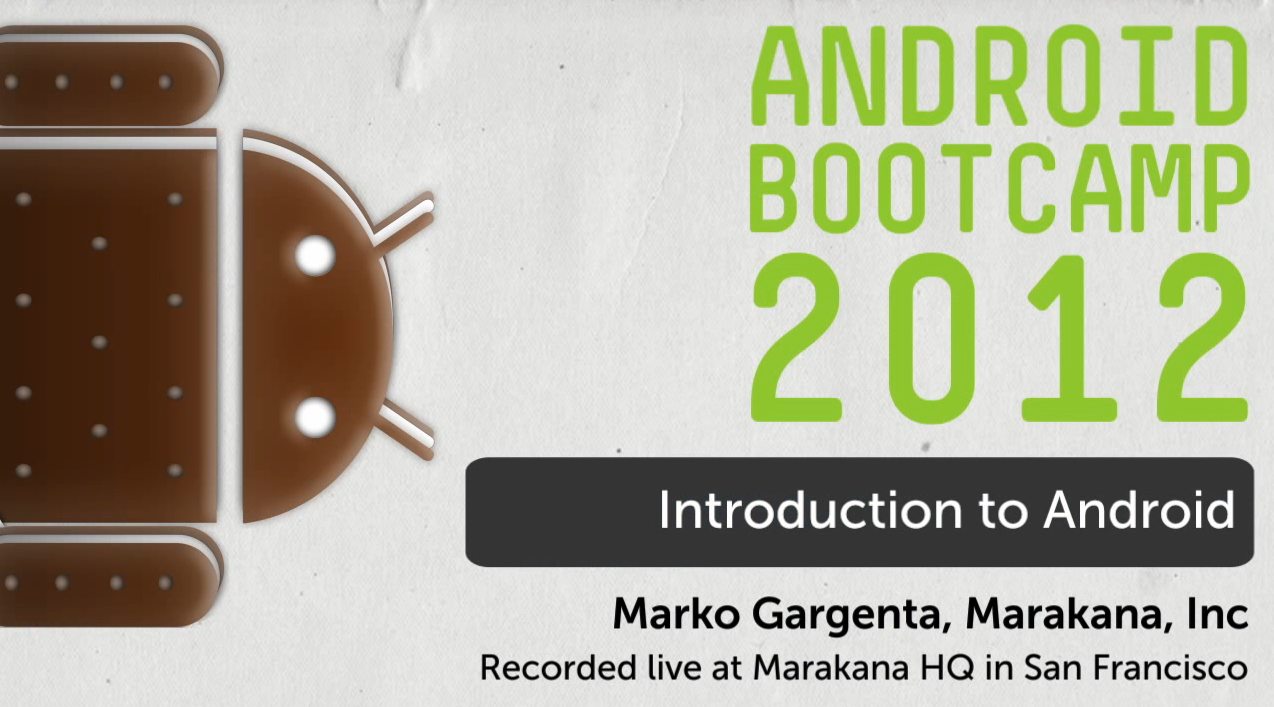
\includegraphics[scale=.14]{marakanabootcamp.png}$\ $
		\raisebox{-.8mm}{
\includegraphics[scale=.332]{marakanabootcampqr.png}}
		
		\vspace{5mm}
		
		{\small\url{http://www.youtube.com/playlist?list=PLE08A97D36D5A255F}}
	\end{slide}
	
	\begin{summary}

		% A {summary} environment can be used to describe the directly      (mh)
		% preceding slide on the handouts. It is responsible for
		% typesetting a smaller version of the slide, with the containing
		% text set next to it (and flowing around it). Without a {summary}
		% environment, the slide itself will not appear in the handouts.

		This is an excellent series of videos that actually taught me a lot of
		the basics (though that was an earlier iteration of the Bootcamp).
		They gave me the idea to use the `live programming' format for this
		presentation.
		
		Just one thing: those videos can be\ldots painfully slow. And 1\sfrac12
		hours will probably be way too fast. I give this presentation only to
		give you a taste of how things look and feel. 
		
		Oh, yeah, and I'm stealing a few slides from them (just a few).
	\end{summary}
	
\subsection{Android Platform}

	\begin{slide}
		\begin{tabular}{|l|l|l|}                                                    \hline
			\bfseries Version       & \bfseries API Level & \bfseries Nickname    \\\hline
			Android 1.0, 1.1        & 1, 2                & Android               \\\hline
			Android 1.5             & 3                   & Cupcake               \\\hline
			Android 1.6             & 4                   & Donut                 \\\hline
			Android 2.0, 2.0.1, 2.1 & 5, 6, 7             & \'Eclair              \\\hline
			Android 2.2             & 8                   & FroYo                 \\\hline
			Android 2.3, 2.3.3      & 9, 10               & Gingerbread           \\\hline
			Android 3.0, 3.1, 3.2   & 11, 12, 13          & Honeycomb             \\\hline
			Android 4.0.2, 4.0.4    & 14, 15              & Ice Cream Sandwich    \\\hline
			Android 4.1.1, 4.2      & 16, 17              & Jelly Bean            \\\hline
			\itshape Android 5.0    & \itshape 18         & \itshape Key Lime Pie \\\hline
		\end{tabular}
	\end{slide}
	
	\begin{summary}
		The API level is the thing developers actually care about. You want to
		\emph{target} a level as high as possible to be able to offer the best new
		features; but you want to \emph{support} a level as low as possible, gracefully
		degrading your app so that people with old phones can still use it.
	\end{summary}
	
	\begin{slide}
		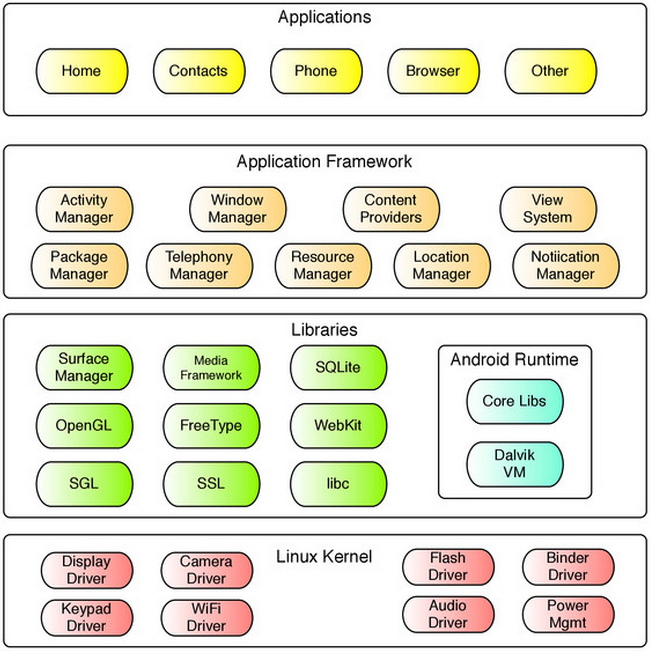
\includegraphics[scale=.28]{androidstack.png}
	\end{slide}
	
	\begin{summary}
		This is very cool. Android is built upon the \emph{Linux Kernel}. Only the kernel,
		mind you.
		
		The \emph{Libraries} on top of it are all open source and optimized for a mobile
		environment. We \emph{don't} care about caching as much, because everything is
		flash memory. We \emph{do} care about battery life.
		
		On top of that, we have the \emph{Application Framework}. This is the only thing app
		developers have access to, and this is what corresponds to a specific `API Level'.
		
		On top of that are your apps. And Google's \emph{apps}. And any app you download
		from Google Play.
	\end{summary}
	
\subsection{Android Programming}
	
	\begin{slide}
		
\includegraphics[scale=.4]{java.jpg}
	\end{slide}
	
	\begin{summary}
		Android programming is Java programming. Most of what you can do with Java, you can do
		with Android. But the `way of working' can sometimes be quite different.
		
		You don't have to worry about creating a \texttt{main()} method, for instance. That's
		all taken care of by the Application Framework. It includes an \emph{event loop}, and
		it is up to you to `react' to many different kinds of events by extending existing
		(abstract) classes and then overwriting specific methods.
	\end{summary}
	
	\begin{slide}
		
\includegraphics[scale=.4]{eclipse.png}
	\end{slide}
	
	\begin{summary}
		You can actually program for Android without any IDE. Everything is available on the
		command line. But Eclipse makes the go work infinitely more smoothly. They've put
		quite some work into the Android Eclipse plugin. You should probably use it. 
	\end{summary}
	
	\begin{slide}
		\huge
		\begin{block}{Main Building Blocks}
			\begin{itemize}
			  \item<1-> Activity
			  \item<2-> Service
			  \item<3-> Broadcast Receiver
			  \item<4-> Content Provider
			  \item<5-> Intent
			\end{itemize}
		\end{block}
	\end{slide}
	
	\begin{summary}[5]

		% When a slide contains multiple overlays / transitions,            (mh)
		% the {summary} environment needs to know which of them to
		% put on the handouts. In this case, it is overlay 5.

		\emph{Activities} are visible screens on the phone. They have layouts, buttons, text
		and that kind of thing. A \emph{Service} is a unit that can run code in the background
		without necesserily having anything visible (by default they don't run in a separate
		thread, though). A \emph{Broadcast Receiver} can pick up all kinds of signals from the
		system, other apps - or itself - and react to them in some way (like notifying other
		parts of the app). A \emph{Content Provider} makes data from your app available to other
		apps, so they can all work with the same data-set. All of these communicate with each
		other by sending \emph{Intents}. In this presentation we only concern ourselves with
		activities, services and intents.
	\end{summary}
	
	\begin{slide}
		\huge
		\begin{block}{Managers}
			\begin{itemize}
			  \item<1-> Media
			  \item<2-> Internet
			  \item<3-> Phone
			  \item<4-> Bluetooth
			  \item<5-> Notifications
			\end{itemize}
		\end{block}
	\end{slide}
	
	\begin{summary}[5]
		Android has a common pattern of exposing the functionality of the device and
		operating system to app developers: \emph{Managers}. This slide lists just a
		few example aspects that can be controlled through Managers.
	\end{summary}
	
	\begin{slide}
		
\includegraphics[scale=.5]{androiddevqr.png}
		
		\vspace{5mm}
		
		{\huge\url{http://developer.android.com}}
	\end{slide}
	
	\begin{summary}
		As an Android developer, there is a single website that will be most important
		to you. The official API reference on the Android Developer website.
	\end{summary}

\section{Hello World!}
	
	\begin{slide}
		{\Huge Create a new}
		
		\vspace{3mm}
		
		{\Huge Android Application Project}
		
		\vspace{3mm}
		
		{\Huge in Eclipse}
	\end{slide}

	% The above slide is the first one without a {summary} environment,     (mh)
	% which will therefore not be inserted in the handouts. But a bit
	% further on, we'll see a command to put it in, anyway.

	\begin{slide}
		{\Huge Explore the GUI Designer}
		
		\vspace{5mm}
		
		\huge
		\begin{minipage}{5cm}
			\begin{itemize}
			  \item Activities
			  \item Layouts
			  \item Widgets
			  \item Toolbars
			  \item Properties
			\end{itemize}
		\end{minipage}
	\end{slide}
	
	\begin{slide}
		{\Huge Create and Run}
		
		\vspace{3mm}
		
		{\Huge Hello~World~0.1}
	\end{slide}
	
	% The commands \showThisSlide, \showPreviousSlide and                   (mh)
	% \showPreviousPreviousSlide are used to typeset smaller versions
	% of the previous three slides, just wide enough so that 3 of them
	% fit next to each other on an A4 handout.
	% 
	% Granted, it's a bit of a silly, limited way to achieve this. I just
	% hacked it together when I lacked time for anything more elegant.
	
	\showPreviousPreviousSlide\showPreviousSlide\showThisSlide
	\vspace{4mm}
	
	\begin{slide}
		{\Huge Explore App Anatomy (files)}
		
		\vspace{5mm}
		
		\huge
		\begin{minipage}{7cm}
			\begin{itemize}
			  \item \verb~Manifest.xml~
			  \item Resources in \verb~res/~
			  \item Java code in \verb~src/~
			  \item (Libraries in \verb~libs/~)
			  \item (Assets in \verb~assets/~)
			\end{itemize}
		\end{minipage}
	\end{slide}
	
	\begin{slide}
		{\Huge Implement Interactivity}
		
		\pause
		
		\vspace{3mm}
		
		{\Huge Hello~World~0.2!}
	\end{slide}
	
	\showPreviousSlide\showThisSlide

\section{A Real App} %%%%%%%%%%%%%%%%%%%%%%%%%%%%%%%%%%%%%%%%%%%%%%%%%%%%%%%%%%%

\subsection{Activities}% % % % % % % % % % % % % % % % % % % % % % % % % % % % %
	
	\begin{slide}
		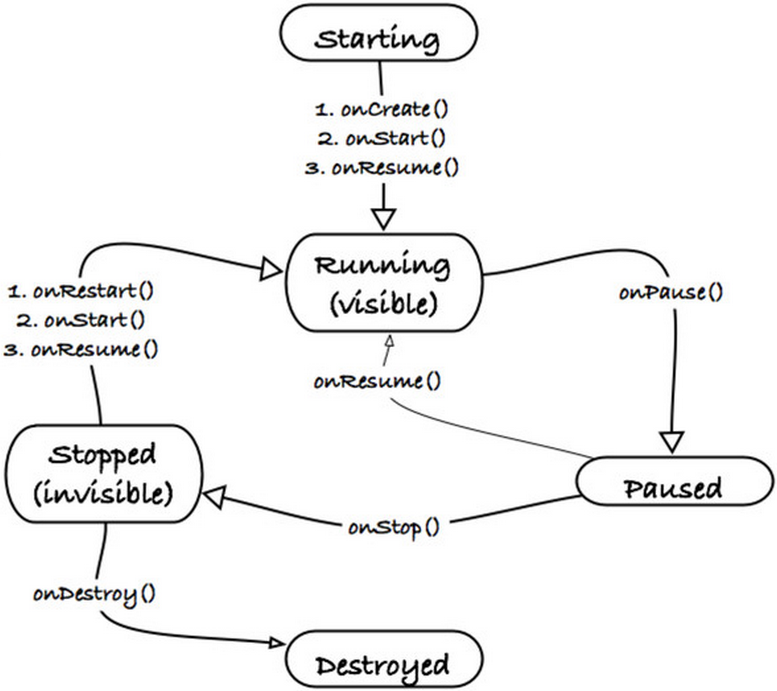
\includegraphics[scale=.25]{activitylifecycle.png}
	\end{slide}
	
	\begin{summary}
		Activities have a well-defined \emph{lifecycle}. App developers cannot directly
		control this lifecycle (merely hint / request), but can dictate how their
		activity behaves on transitions between phases. For this purpose there is a set
		of methods that you can overwrite when you inherit from the \verb~Activity~
		class. This way you can always request or release resources, save data
		or do anything else to make sure your activity behaves properly no matter
		what the user or the operating system does.
	\end{summary}
	
	\begin{slide}
		{\Huge Use Logcat; Live Logcat}
		
		\vspace{5mm}
		
		\huge
		\begin{minipage}{7cm}
			\begin{itemize}
			  \item Log Activity Lifecycle
			  \item \verb~TAG~, you're it!
			\end{itemize}
		\end{minipage}
	\end{slide}
	
	\begin{slide}
		{\Huge Create a `Real' App}
	\end{slide}
	
	\begin{slide}
		{\Huge Our Stages of Development}
		
		\vspace{5mm}
		
		\Large
		\begin{minipage}{11cm}
			\begin{itemize}
			  \item Create an \verb~Activity~ for scheduling the alarm \pause
			  \item Test; Log \pause
			  \item Create a \verb~Service~ that can trigger an alarm \pause
			  \item Test; Log \pause
			  \item Connect the two with \verb~Intent~s \pause
			  \item Meh\ldots It probably works\ldots
			\end{itemize}
		\end{minipage}
	\end{slide}
	
	% As you can see, the \showThisSlide command (and family) also          (mh)
	% accept an overlay number.
	
	\showPreviousPreviousSlide\showPreviousSlide\showThisSlide[6]
	\vspace{4mm}
	
	\begin{slide}
		{\Huge Create an \verb~Activity~}
		
		\vspace{3mm}
		
		{\Huge for Scheduling the Alarm}
		
		\pause
		
		\vspace{5mm}
		
		\Huge
		\begin{minipage}{5cm}
			\begin{itemize}
			  \item Message \pause
			  \item Frequency \pause
			  \item Period
			\end{itemize}
		\end{minipage}
		
		\pause
		
		\vspace{5mm}
		
		{\Huge Add to \verb~manifest.xml~!}
	\end{slide}
	
	\begin{slide}
		{\Huge Create a \verb~Service~}
		
		\vspace{3mm}
		
		{\Huge that can Trigger an Alarm}
		
		\pause
		
		\vspace{1cm}
		
		{\Huge Add to \verb~manifest.xml~!}
	\end{slide}
	
	\showPreviousSlide[5]\showThisSlide[2]

\subsection{Services}% % % % % % % % % % % % % % % % % % % % % % % % % % % % % %
	
	\begin{slide}
		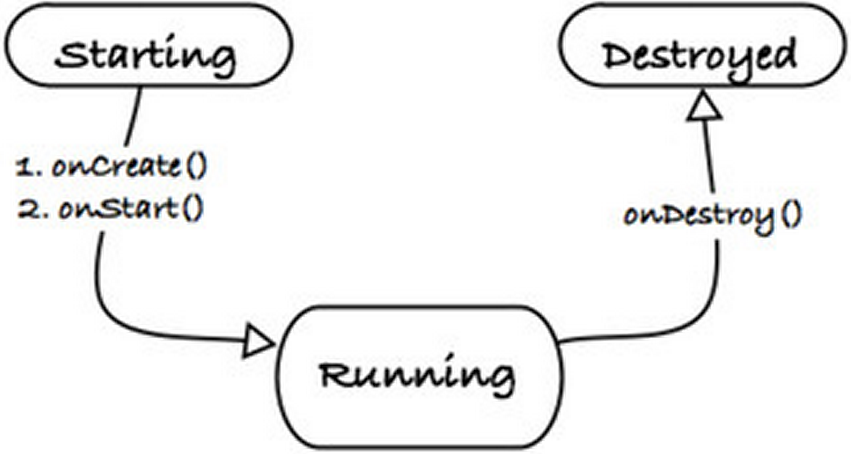
\includegraphics[scale=.3]{servicelifecycle.png}
	\end{slide}
	
	\begin{summary}
		Like activities, services also have a lifecycle, but a much easier one.
		They are created, started and then destroyed. Nonetheless, it is
		important that you prepare your service to be killed at any time when
		the OS decides that it needs to kill it to reallocate resources.
	\end{summary}
	
	\begin{slide}
		{\Huge Log \verb~Service~ Lifecycle}
	\end{slide}
	
	\begin{slide}
		{\Huge Try \verb~IntentService~;}
		
		\vspace{3mm}
		
		{\Huge it's easier\ldots}
	\end{slide}
	
	\begin{slide}
		{\Huge Call a \verb~Notification~}
		
		\vspace{3mm}
		
		{\Huge using \verb~NotificationManager~}
	\end{slide}
	
	\showPreviousPreviousSlide\showPreviousSlide\showThisSlide
	\vspace{4mm}
	
	\begin{slide}
		{\Huge Schedule the Notification}
		
		\vspace{3mm}
		
		{\Huge using \verb~AlarmManager~}
	\end{slide}
	
	\showThisSlide

\subsection{Intents} % % % % % % % % % % % % % % % % % % % % % % % % % % % % % %

	\begin{slide}
		{\Huge Send our Alarm Information}
		
		\vspace{3mm}
		
		{\Huge using Intent \verb~extras~}
	\end{slide}
	
	\begin{slide}
		{\Huge Do we have Time?}
		
		\pause
		
		\vspace{3mm}
		
		{\Huge Feature Ideas?}
	\end{slide}
	
	\showPreviousSlide\hfill\showThisSlide[2]
	
\semisection{Conclusion} %%%%%%%%%%%%%%%%%%%%%%%%%%%%%%%%%%%%%%%%%%%%%%%%%%%%%%%
	
	\begin{slide}
		\Huge
		\url{www.mhelvens.net}
	\end{slide}
	
	\begin{summary}
		Thanks for reading!
	\end{summary}
	
	\mode<article>{

		% You can use \mode<article> whenever you need it to make           (mh)
		% content appear on the handouts only. This is not always
		% needed (with \showThisSlide, for example), but it is the
		% best way to be sure you won't mess up your slides.

		\newpage\topskip0pt
		\vspace*{\fill}
		\begin{center}
			\Huge \tt intentionally (almost) empty
		\end{center}
		\vspace*{\fill}
	}
	
%%%%%%%%%%%%%%%%%%%%%%%%%%%%%%%%%%%%%%%%%%%%%%%%%%%%%%%%%%%%%%%%%%%%%%%%%%%%%%%%
\end{document}                                                                 %
%%%%%%%%%%%%%%%%%%%%%%%%%%%%%%%%%%%%%%%%%%%%%%%%%%%%%%%%%%%%%%%%%%%%%%%%%%%%%%%%
